\question{Спонтанные и индуцированные переходы. Коэффициенты Эйнштейна.}

При индуцированных переходах квантовая система может переводиться из одного 
энергетического состояния в другое \ref{img1.1} как с поглощение энергии 
электромагнитного поля (переход с нижнего на верхний), так и с излучением 
электромагнитной энергии (переход с верхнего на нижний).

\begin{figure}[h!]
	\center
	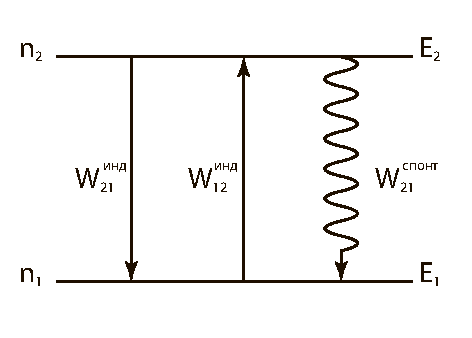
\includegraphics[width=.4\textwidth]{image1_1} \\
	\caption{Схема двух уровней энергии \( E_2 > E_1 \)}
	\label{img1.1}
\end{figure}

Индуцированные переходы обладают следующими важными свойствами.

Во-первых, вероятность индуцированных переходов отлична от нуля только для 
внешнего поля резонансной частоты, энергия которого \( h\nu \) совпадает с 
разностью энергий двух изолированных состояний (\( E_2 \) и \( E_1 \), где 
индекс 2 относится к большей энергии, а 1 -- к меньшей). Это условие 
соответствия постулату Бора:
\[
	h\nu = E_2 - E_1
\]

Во-вторых, кванты электромагнитного поля, излученные при индуцированных 
переходах, полностью тождественны квантам поля, вызвавшего эти переходы. 
То есть внешнее электромагнитное поле и поле, созданное при индуцированных 
переходах, имеют одинаковые частоту, фазу, поляризацию и направление 
распространения -- они тождественны.

В-третьих, вероятность индуцированных переходов в единицу времени 
пропорциональна плотности энергии внешнего поля в единичном спектральном 
интервале:
\[
	W_{12}^\text{инд} = B_{12}\rho_\nu
\]
\[
	W_{12}^\text{инд} = B_{12}\rho_\nu
\]

где \( B_{12} \) и  \( B_{21} \) -- коэффициенты Эйнштейна для индуцированного 
поглощения и излучения соответственно, а порядок индексов 1 и 2 указывает 
направление перехода.

Таким образом индуцированное излучение -- это излучение вынужденное, 
стимулированное внешним излучением. 

Кроме индуцированного внешним полем, существует и самопроизвольное испускание 
излучения. Атомы, находящиеся в верхнем энергетическом состоянии, могут 
совершать спонтанные переходы в нижнее состояние. Эти переходы 
самопроизвольны. Происходящий при спонтанном излучении распад верхнего 
энергетического состояния подобен радиоактивному распаду неустойчивого ядра. 
Вероятность спонтанных переходов не зависит от внешнего электромагнитного 
поля, акты спонтанного излучения никак не связаны с внешним полем. Поэтому 
спонтанное излучение некогерентно по отношению к внешнему полю и играет 
роль собственных шумов. Кроме того, спонтанное излучение опустошает верхний 
энергетический уровень, способствуя возвращению атома в нижнее энергетическое 
состояние.

Спонтанное излучение является эффектом принципиально квантовым, не допускающим 
классической трактовки. В классической механике метастабильное состояние, 
обладающее большей энергией по отношению к некоторому основному устойчивому 
состоянию, в отсутствие внешних возмущений может жить бесконечно долго. В 
квантовой области такое метастабильное состояние спонтанно распадается с 
некоторой отличной от нуля средней скоростью.

...